\chapter{Impedance Transformation and Power Transfer}\label{lec:lec6}
In our previous chapter, we investigated the Standing Wave Pattern on a transmission line and also an important parameter which is the voltage standing wave ratio VSWR, (which is the ratio of the maximum voltage seen on the transmission line to the minimum voltage seen on the transmission line).

In this chapter, we will study the impedance transformation on a lossless
transmission line and we will establish some of the very important characteristics of impedance transformation on a lossless transmission line. After which, we will proceed to an important calculation of Power Transfer to the Load and also the expression for $V^{+}$.
\section{Transformation on a Lossless Transmission Line}
Recall that, the impedance transformation relationship for any point is given as:
\begin{align*}
\footnotemark[1]Z(l) = Z_o\left\lbrace \frac{Z_L\cosh(\gamma l) + Z_o\sinh(\gamma l)}{Z_o\cosh(\gamma l) + Z_L\sinh(\gamma l)}\right\rbrace 
\end{align*}
\footnotetext[1]{$Z(l)$ is the impedance at any point on the line}
\footnotetext[2]{$\bar{Z}(l)$ is the normalized impedance at any point on the line}
\begin{align*}
\footnotemark[2]\bar{Z}(l) = \left\lbrace \frac{\bar{Z}_L\cosh(\gamma l) + \sinh(\gamma l)}{\bar{Z}_L\sinh(\gamma l) + \cosh(\gamma l)}\right\rbrace 
\end{align*}
if $\bar{Z_L} = 1$ i.e $Z_L = Z_o$ and $\bar{Z}(l) = 1 \rightarrow  Z(l) = Z_o$

For a lossless Transmission Line,$\gamma=j\beta$ where
\begin{align*}
\cosh\gamma l = \frac{e^{\gamma l} + e^{-\gamma l}}{2} \quad and \quad \sinh\gamma l = \frac{e^{\gamma l} - e^{-\gamma l}}{2}
\end{align*}
so,
\begin{align*}
\cosh\gamma l= \cosh(j\beta l)=\frac{e^{j \beta l} + e^{-j \beta l}}{2}=\cos(\beta l)
\end{align*}
And
\begin{dmath*}
\sinh\gamma l=\sinh(j\beta l) = \frac{e^{j \beta l}-e^{-j\beta l}}{2} = j\left( \frac{e^{j\beta l}-e^{-j\beta l}}{2j}\right) =j\sin(\beta l)
\end{dmath*}

Therefore impedance transformation relationship for a lossless transmission line is given as;
\begin{equation}
\bar{Z}(l) = \left\lbrace \frac{\bar{Z}_L\cos(\beta l) + j\sin(\beta l)}{\cos(\beta l) + j\bar{Z}_L\sin(\beta l)}\right\rbrace
\label{eqn:charimp}
\end{equation}
$Z_o$ is a real quantity for a lossless transmission line same as:
\begin{equation}
\bar{Z}(l) = \left\lbrace \frac{\bar{Z}_L\cos(\beta l) + j\sin(\beta l)}{\cos(\beta l) + j\bar{Z}_L\sin(\beta l)}\right\rbrace
\label{eqn:charimpnorm}
\end{equation}
With this impedance transformation relationship, we can establish some very important characteristics of the transmission line. When we move on a transmission line a distance of $\frac{\lambda}{2}$ (half wave length), the voltage standing wave characteristics repeat itself, so if we take a ratio of voltage and current at a certain location, we expect that this characteristic will repeat at $\frac{\lambda}{2}$.

Moving $\frac{\lambda}{4}$ from the point of $R_{\max}$ and $R_{\min}$, should bring something interesting. Similarly, if we terminate the line into its characteristics impedance, the impedance measured at any point equals to the characteristics impedance. So we have three important points we can draw from this.

Lets show with proof these three characteristics.
\subsection{Normalized impedance value repeat every $\frac{\lambda}{2}$ distance}
Lets say at $l$ we have maximum or minimum impedance, then moving $l=\frac{\lambda}{2}$ from that point we should get same impedance again!

At location $l$, Impedance $= \bar{Z}(l)$,
\begin{figure}[h]
\centering
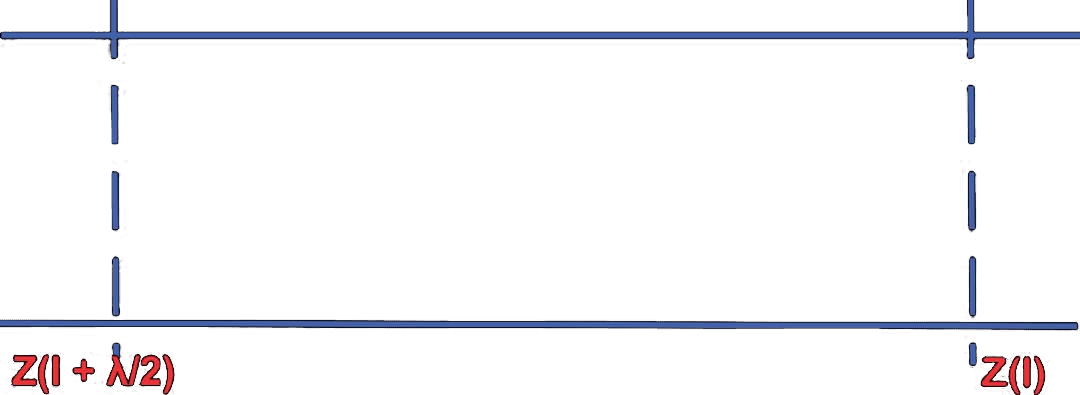
\includegraphics[width=0.8\linewidth]{./graphics/6}
\caption{Z($l$) over distance $\frac{\lambda}{2}$}
\label{fig:astyuif}
\end{figure}

At location ${\left(l+\frac{\lambda}{2}\right)}$, Impedance $= \bar{Z}\left(l+\frac{\lambda}{2}\right)$ substituting ${\left(l+\frac{\lambda}{2}\right)}$ for $l$ in equation~\ref{eqn:charimp}, we get: 
\begin{align*}
\bar{Z}\left(l+\frac{\lambda}{2}\right) = \left\lbrace \frac{\bar{Z}_L \cos(\beta \left(l+\frac{\lambda}{2}\right)) + j\sin(\beta \left(l+\frac{\lambda}{2}\right))}{\cos(\beta \left(l+\frac{\lambda}{2}\right)) + j\bar{Z}_L \sin(\beta \left(l+\frac{\lambda}{2}\right))}\right\rbrace 
\end{align*}
Since \footnote{$\beta$ represents phase constant}$\beta$ = $ \frac{2\pi}{\lambda}$, therefore,
\begin{dmath*}
\beta\left(l+\frac{\lambda}{2}\right)=\frac{2\pi}{\lambda}\left(l+\frac{\lambda}{2}\right)=\frac{2\pi}{\lambda}l+\pi=\beta l+\pi
\end{dmath*}
\begin{align*}
\bar{Z}\left(l+\frac{\lambda}{2}\right) = \left\lbrace \frac{\bar{Z}_L\cos(\beta l+\pi) + j\sin(\beta l+\pi)}{\cos(\beta l+\pi) + j\bar{Z}_L\sin(\beta l+\pi)}\right\rbrace 
\end{align*}
But 
\[
\cos(\beta l+\pi)=-\cos(\beta l)$ and $\sin(\beta l+\pi)=-\sin(\beta l)
\] 
\begin{dmath*}
\bar{Z}\left(l+\frac{\lambda}{2}\right)=\left\lbrace \frac{-\bar{Z}_L \cos(\beta l) - j\sin(\beta l)}{-\cos(\beta l) - j\bar{Z}_L \sin(\beta l)}\right\rbrace = \left\lbrace \frac{\bar{Z}_L \cos(\beta l) + j\sin(\beta l)}{\cos(\beta l) + j\bar{Z}_L \sin(\beta l)}\right\rbrace\;\;\equiv\bar{Z}(l)
\end{dmath*} 
This is same as original formula obtained for $\bar{Z}(l)$.

Hence $\bar{Z}\left(l+\frac{\lambda}{2}\right)=\bar{Z}(l)$, which proves that impedance repeat itself at $\frac{\lambda}{2}$.

In other words, no matter the length of the transmission line, modulus $\frac{\lambda}{2}$ is  a special information which is available from the impedance relationship.

\subsection{Normalized impedance inverts at every $\frac{\lambda}{4}$ distance}
If we move a distance of $\frac{\lambda}{4}$, we move from a maximum to minimum impedance and vice versa.

At location $l, \textnormal{Impedance}=\bar{Z}(l)$.

Then at location ${(l+\frac{\lambda}{4})}$, Impedance  $=\bar{Z}(l+\frac{\lambda}{4})$. Substituting ${(l+\frac{\lambda}{4})}$ for $l$ in equation~\ref{eqn:charimp}, we get:
\begin{align*}
\bar{Z}\left(l+\frac{\lambda}{4}\right) = \left\lbrace \frac{\bar{Z}(l)\cos(\beta (l+\frac{\lambda}{4})) + jsin(\beta (l+\frac{\lambda}{4}))}{\cos(\beta (l+\frac{\lambda}{4})) + j\bar{Z}(l)\sin(\beta (l+\frac{\lambda}{4}))}\right\rbrace 
\end{align*}
Where 
\begin{dmath*}
\beta(l + \frac{\lambda}{4})=\beta l + \frac{2\pi}{\lambda} \cdot \frac{\lambda}{4} = \beta l + \frac{\pi}{2}
\end{dmath*}
\begin{align*} 
\bar{Z}\left(l+\frac{\lambda}{4}\right) = \left\lbrace \frac{\bar{Z}(l)\cos(\beta l + \frac{\pi}{2}) + j\sin(\beta l + \frac{\pi}{2})}{\cos(\beta l + \frac{\pi}{2}) + j\bar{Z}(l)\sin(\beta l + \frac{\pi}{2})}\right\rbrace
\end{align*}
But $\cos(\beta l + \frac{\pi}{2})= -\sin(\beta l), \sin(\beta l+\frac{\pi}{2})=\cos(\beta l)$
\begin{align*} 
\bar{Z}\left(l+\frac{\lambda}{4}\right) = \left\lbrace \frac{-\bar{Z}(l)\sin(\beta l) + j\cos(\beta l)}{-\sin(\beta l) + j\bar{Z}(l) \cos(\beta l)}\right\rbrace
\end{align*}
\begin{dmath*}
\bar{Z}\left(l+\frac{\lambda}{4}\right) =\frac{j}{j} \left\lbrace \frac{\cos(\beta l) + j\bar{Z}(l)\sin(\beta l)}{\bar{Z}(l)\cos(\beta l) + j\sin(\beta l)}\right\rbrace 
= \frac{1}{\left\lbrace \frac{\bar{Z}(l)\cos(\beta l) + j\sin(\beta l)}{\cos(\beta l) + j\bar{Z}(l)\sin(\beta l)}\right\rbrace} 
=\frac{1}{\bar{Z}(l)}
\end{dmath*}
We can draw an observation that for every $\frac{\lambda}{4}$ distance moved, the normalized impedance inverts itself\footnote{Note the word \textbf{normalized}, it is not absolute impedance}. If absolute impedance is inverted, it is \textbf{admittance}\index{admittance}. The normalized impedance does not have a unit, it is dimensionless. So if I have an impedance greater than $Z_o$ along a transmission line, after $\frac{\lambda}{4}$ distance, it becomes less than $Z_o$ because the normalized impedance is the inverse of the one at previous location. So at $\frac{\lambda}{4}$ distance, impedance inverts after another $\frac{\lambda}{4}$ again it re-inverts becoming the original impedance, which is equivalent to repeating itself at $\frac{\lambda}{2}$ distance. 

Hence, when we talk about the periodicity of the impedance on the transmission line, at $\frac{\lambda}{2}$ the absolute or normalized impedance repeats itself, whereas every distance of $\frac{\lambda}{4}$, the normalized impedance inverts itself. Next on is the study of impedance matching characteristics; this property is used extensively for finding out the impedance transformation which can match impedance on transmission line.

\subsection{The matching condition characteristics}
If the transmission line is terminated by its characteristics impedance, then the impedance seen at every point on the transmission line is equal to the characteristics impedance. So if $Z_L=Z_o$. This implies that $\bar{Z}_L= \frac{Z_L}{Z_o}=1$. Then equation~\ref{eqn:charimp} becomes:
\begin{dmath*}
\bar{Z}(l) = \left\lbrace\frac{\bar{Z}_L\cos\beta l + j\sin\beta l}{\cos\beta l + j\bar{Z}_L\sin\beta l}\right\rbrace = \left\lbrace \frac{\cos\beta l + j\sin\beta l}{\cos\beta l + jsin\beta l}\right\rbrace = 1
\end{dmath*}
Therefore, irrespective of the length of the transmission line, if the line is terminated in its characteristics impedance, then the impedance seen at every point on the transmission line is equal to the characteristics impedance. This means that once a line is terminated in its characteristics impedance, there is no need to compute the impedance transformation on the line, we can use any length of transmission and the impedance will always be the same along the length of the line. 

$Z_L=Z_o$ i.e when reflection coefficient is zero, there is no reflected wave on the transmission line and we have only forward traveling wave on the transmission line. Forward traveling wave always see an impedance which is equal to the characteristics impedance. This result is not new, it is what we had discussed earlier when we talked about transmission line and that was, if a line is terminated in its characteristic impedance, the impedance seen at every point on the transmission line is equal to the characteristics impedance. 

So these are the three very important characteristics of a lossless transmission line.
\begin{enumerate}[(i)]
\item Impedance transformation repeats at every $\frac{\lambda}{2}$ distances.
\item Normalized impedance inverts at every $\frac{\lambda}{4}$ distance.
\item Finally if the line is terminated in its characteristics impedance, the impedance seen at every point of the line is equal to the characteristics impedance.
\end{enumerate}
With this understanding of impedance transformation, now we can go to Power Transfer Calculation of the transmission line.

\section{Power Transfer on Transmission Line}
Initially, our idea was to transfer power from generator to load effectively. In the lossless case, it should be that all generator power is completely transferred to the load. However, we have seen that if the impedance is not equal to the characteristics impedance, then there will always be reflection on the transmission line and whatever energy the generator supplies, part of this energy will get reflected back to the generator. Now when we talk about matching condition\index{matching condition} or maximum power transfer condition\index{matching power transfer condition}, there are two cases to consider;
\begin{enumerate}[(i)]
\item When the power is generated by the generator, it should be maximally transfered to the load.
\item When the reflected power comes back to generator, the generator is not capable of absorbing power, so when the reflected power comes back with a different amplitude and phase, it negatively affects the generator's performance (destructive interference). So it is desirable that the generator should not see any power coming back at it.
\end{enumerate}
For these two reasons that the generator power should be completely delivered to the load and that no reflected power should come back to the generator, we must make sure always that the impedance which the generator sees is always equal to the characteristics impedance. We will study these two issues later but let's study a general case and suppose we have a transmission line which is connected to a generator at  one end and a load at the other end. Then, \emph{how much power will be delivered to the load?} Again using the voltage and current equation, we can write down power at the location of the load i.e power delivered to the load will be given as follows.

At load end, $L=0$ therefore, $e^{-2\beta (l)} = e^{-2\beta (0)}$
\begin{align*}
V(0) &= V^{+} \left\lbrace {1 + \Gamma_L e^{-2\beta(0)}}\right\rbrace\\ 
&= V^{+}\left\lbrace 1 +\Gamma_L \right\rbrace\\
I(0) &= \frac{V^{+}}{Z_o} \left\lbrace{1 - \Gamma_L e^{-2\beta(0)}}\right\rbrace\\ 
&= \frac{V^{+}}{Z_o}\left\lbrace1 -\Gamma_L \right\rbrace
\end{align*}
So from the general voltage and current relationship on the transmission line we have found  out the voltage and current values at load end.

$Z_o= $ real for a lossless line, thus the conjugate of the current equation at the load end is:
\begin{align*}
I^\ast (0) =\frac{V^{+ (\ast )}}{Z_o}\left\lbrace 1 -\Gamma_L \right\rbrace
\end{align*}

Power delivered to load.
\begin{dmath*}
P = \frac{1}{2}\mathfrak{Re}\left\lbrace V(0) I^\ast(0) \right\rbrace= \frac{1}{2}\mathfrak{Re}\left\lbrace V^+(1+\Gamma_L) \times\frac{V^{+(\ast)}}{Z_o} (1-\Gamma_L)\right\rbrace
\end{dmath*}
\begin{equation}
P = \frac{1}{2} \frac{|V^+|^2}{Z_o} \left\lbrace 1 -|\Gamma_L|^2 \right\rbrace\footnotemark
\end{equation}
\footnotetext{
Given $V=a + jb  \quad \quad V^\ast=a-jb$

Then, $V\times V^\ast = (a + jb)(a-jb)= a^2-jab + jab +(jb)(-jb)=a^2 + b^2$

$|V|= \sqrt{a^2 + b^2}$ thus, $|V|^2 = a^2 + b^2$

This implies that $|V|^2 = V \times V^* $}
$\Gamma_L$ is a real value since it is the absolute value taken here.

Recall that,
\begin{align*}\Gamma_L = \frac{ Z_L -Z_o }{ Z_L + Z_o }.
\end{align*}

Once load impedance is known, the reflection coefficient at load end is known. Then we can calculate modulus of reflection coefficient so that the power delivered to the load can be calculated if $V^+$ is known. How do we find $V^+ ? $ From the relationship here, if we know the amplitude of the forward traveling wave as well as the load impedance, we can calculate the power from the circuit perspective point of view. We can use a different argument in arriving at the same answer. That is on the transmission line the power supplied from generator, in the form of a traveling wave goes towards the load and we already said that traveling wave always see impedance equal to characteristics impedance. So if the traveling wave has amplitude $V^+$, it is as if this wave is supplying the power to $Z_o$ in the lossless case. So one can say now that  a wave having amplitude $V^+$ going forward direction sees impedance $Z_o$.

Power carried by forward wave:  
\begin{align*}
P_{\textnormal{for}} = \frac{1}{2} \frac{{|V|^+}^2}{Z_o}
\end{align*}
When this gets to the load, part of the energy will get reflected back, and this backward traveling wave has amplitude $V^-$ which also sees characteristics impedance.

The power carried by this wave:
\begin{align*}
P_{\textnormal{ref}} = \frac{1}{2}\frac{{|V^-|}^2}{Z_o}
\end{align*}
which is the power reflected by load in the backward wave.

Therefore,
\begin{align*} 
\textnormal{Power delivered to load}, P\\
=& \textnormal{Power transferred to load}\\
&- \textnormal{Power reflected}\\
=& \frac{1}{2} \frac{{|V^+|}^2}{Z_o} -\frac{1}{2} \frac{{|V^-|}^2 }{Z_o}\\
=& \frac{1}{2} \left\lbrace \frac{{|V^+| }^2}{Z_o} -\frac{ {|V^-|}^2 }{Z_o} \right\rbrace\\
=& \frac{1}{2} \frac{{|V^+|}^2}{Z_o} \left\lbrace 1 - {
\begin{vmatrix}
\frac{V^-}{V^+}
\end{vmatrix}^2}\right\rbrace
\end{align*}
Recall that $\Gamma_L =\frac{V^-}{V^+}$.
\begin{align*}
P_L=\frac{1}{2} \frac{{|V^+|}^2}{Z_o} \left\lbrace 1 - { \Gamma_L }^2 \right\rbrace.
\end{align*}
So when we compute the power transfer on a transmission line, it is either done using circuit theory concept or wave theory concept. Thus we have found the real part i.e the power actually supplied to the load. One then asks \emph{how do we calculate for complex part or put differently, how do we compute the complex power at any location on the transmission line?}. 

If we calculate the power flow along any point on the transmission line not necessarily at the load end, what will that indicate? To test that theory, let's get the voltage and current at any arbitrary location on the transmission line i.e
\begin{align*} 
V(l) = V^+ e^{j\beta l} \left\lbrace 1 + \Gamma_L e^{-j2\beta l} \right\rbrace,\\ 
I(l) = \frac{V^+}{Z_o} e^{j\beta l} \left\lbrace 1 - \Gamma_L e^{-j2\beta l} \right\rbrace
\end{align*}
Complex Power at location $l$ is thus given as:
\begin{dmath*}
P(l) = \frac{1}{2} (V I^\ast) 
= \frac{1}{2} \left(V^+ e^{j\beta l} \left\lbrace 1 + \Gamma_L e^{-j2\beta l} \right\rbrace \right) \times \left(\frac{V^+}{Z_o} e^{-j\beta l} \left\lbrace 1 - \Gamma_L e^{j2\beta l} \right\rbrace\right)
=\frac{1}{2} \frac{{|V^+|}^2}{Z_o} \left( 1 + \Gamma_L e^{-j2\beta l}\right)\left(1 - \Gamma e^{j2\beta l}\right)
= \frac{1}{2} \frac{{|V^+|}^2}{Z_o}\left(1 - \Gamma_L e^{j2\beta l} + \Gamma_L e^{-j2\beta l} - {|\Gamma_L|^2}\right)
=\frac{1}{2} \frac{{|V^+|}^2}{Z_o}\left\lbrace 1 - {|\Gamma_L|}^2 - \Gamma_L \left(e^{j2\beta l} - e^{-j2\beta l}\right)\right\rbrace
\end{dmath*}
Recall, \( \jmath2\sin\theta = {e}^{\jmath\theta} - {e}^{\jmath\theta}\), so,
\begin{dmath} 
P(l) = \frac{1}{2} \frac{{|V^+|}^2}{Z_o}\left\lbrace 1 - {|\Gamma_L|}^2 - j2\Gamma_L \sin(2\beta l)\right\rbrace
= \frac{1}{2} \frac{{|V^+|}^2}{Z_o}\left\lbrace 1 - {|\Gamma_L|}^2 - \mathfrak{Im}\lbrace\Gamma_L{e}^{-j2\beta l}\rbrace\right\rbrace
\end{dmath}
Thus, given the complex power, the real part is $1 - {|\Gamma_L}|^2$ which is the resistive power, and the imaginary part is $ j2\Gamma_L \sin(2\beta l) = \mathfrak{Im}\lbrace\Gamma_L{e}^{-j2\beta l}\rbrace$ which is the reactive power.
 
Therefore, at any location of the transmission line, the power is complex, the interesting thing to note is that the resistive power at any point is equal to the power which we earlier calculated that is delivered to the load end. So for a lossless line the resistive power at any point along the line is the same as the power which is delivered to the load\footnote{
This can be explained with the line of throught that the resistive power finally gets to the load if the line is lossless, since there is no absorption of power at any point along the line and so all the resistive power gets to the load because the load is the part where you have resistive component and power can be  absorbed in that location.
}. Hence at any point on the transmission line, power transfer of the resistive part is completely delivered to the load and as such the resistive power which is the actual power flow should be independent of any location on the line.

However the reactive power is a function of $l$, which shows the energy stored at different location along the transmission line. Now we have two parts when we calculate the power on a transmission line. \emph{There is a resistive power which is a measure of power flow which ultimately gets delivered to the load and the reactive power which measures the amount energy storage at different location along the line and depends on the value of voltage and current at that location.} Recall that the voltage and current equations are standing waves and thus the energy stored also varies at different location along the transmission line. Therefore, in conclusion, the reactive power will vary at different locations across the line while the resistive power which is the power delivered to the load will be independent of location of the transmission line.

\section{Evaluation of $\mathbf{V^{+}}$} 
So far, our transmission line analysis (voltage and current equations, impedance transformation, power transfer analysis and so on) has been derived in terms of $V^+$. $V^+$ is a final arbitrary constant in the solution of the differential equation of transmission line that we are yet to evaluate. It is the amplitude of the incident voltage, which we have assumed in known a priori. Now the question is \emph{how do we evaluate $V^{+}$?}.

Considering the circuit in figure~\ref{fig:qwerrtt}, $Z_L$ is transformed to $Z^{'}_L$, from position BB' to AA'. $Z^{'}_L$ is the impedance of the load as seen by the generator end. With $Z_L$ transformed to $Z^{'}_L$, the whole circuit is reduced to a lump circuit as shown in figure~\ref{fig:qwerrtt}.
\begin{figure}[h]
\centering
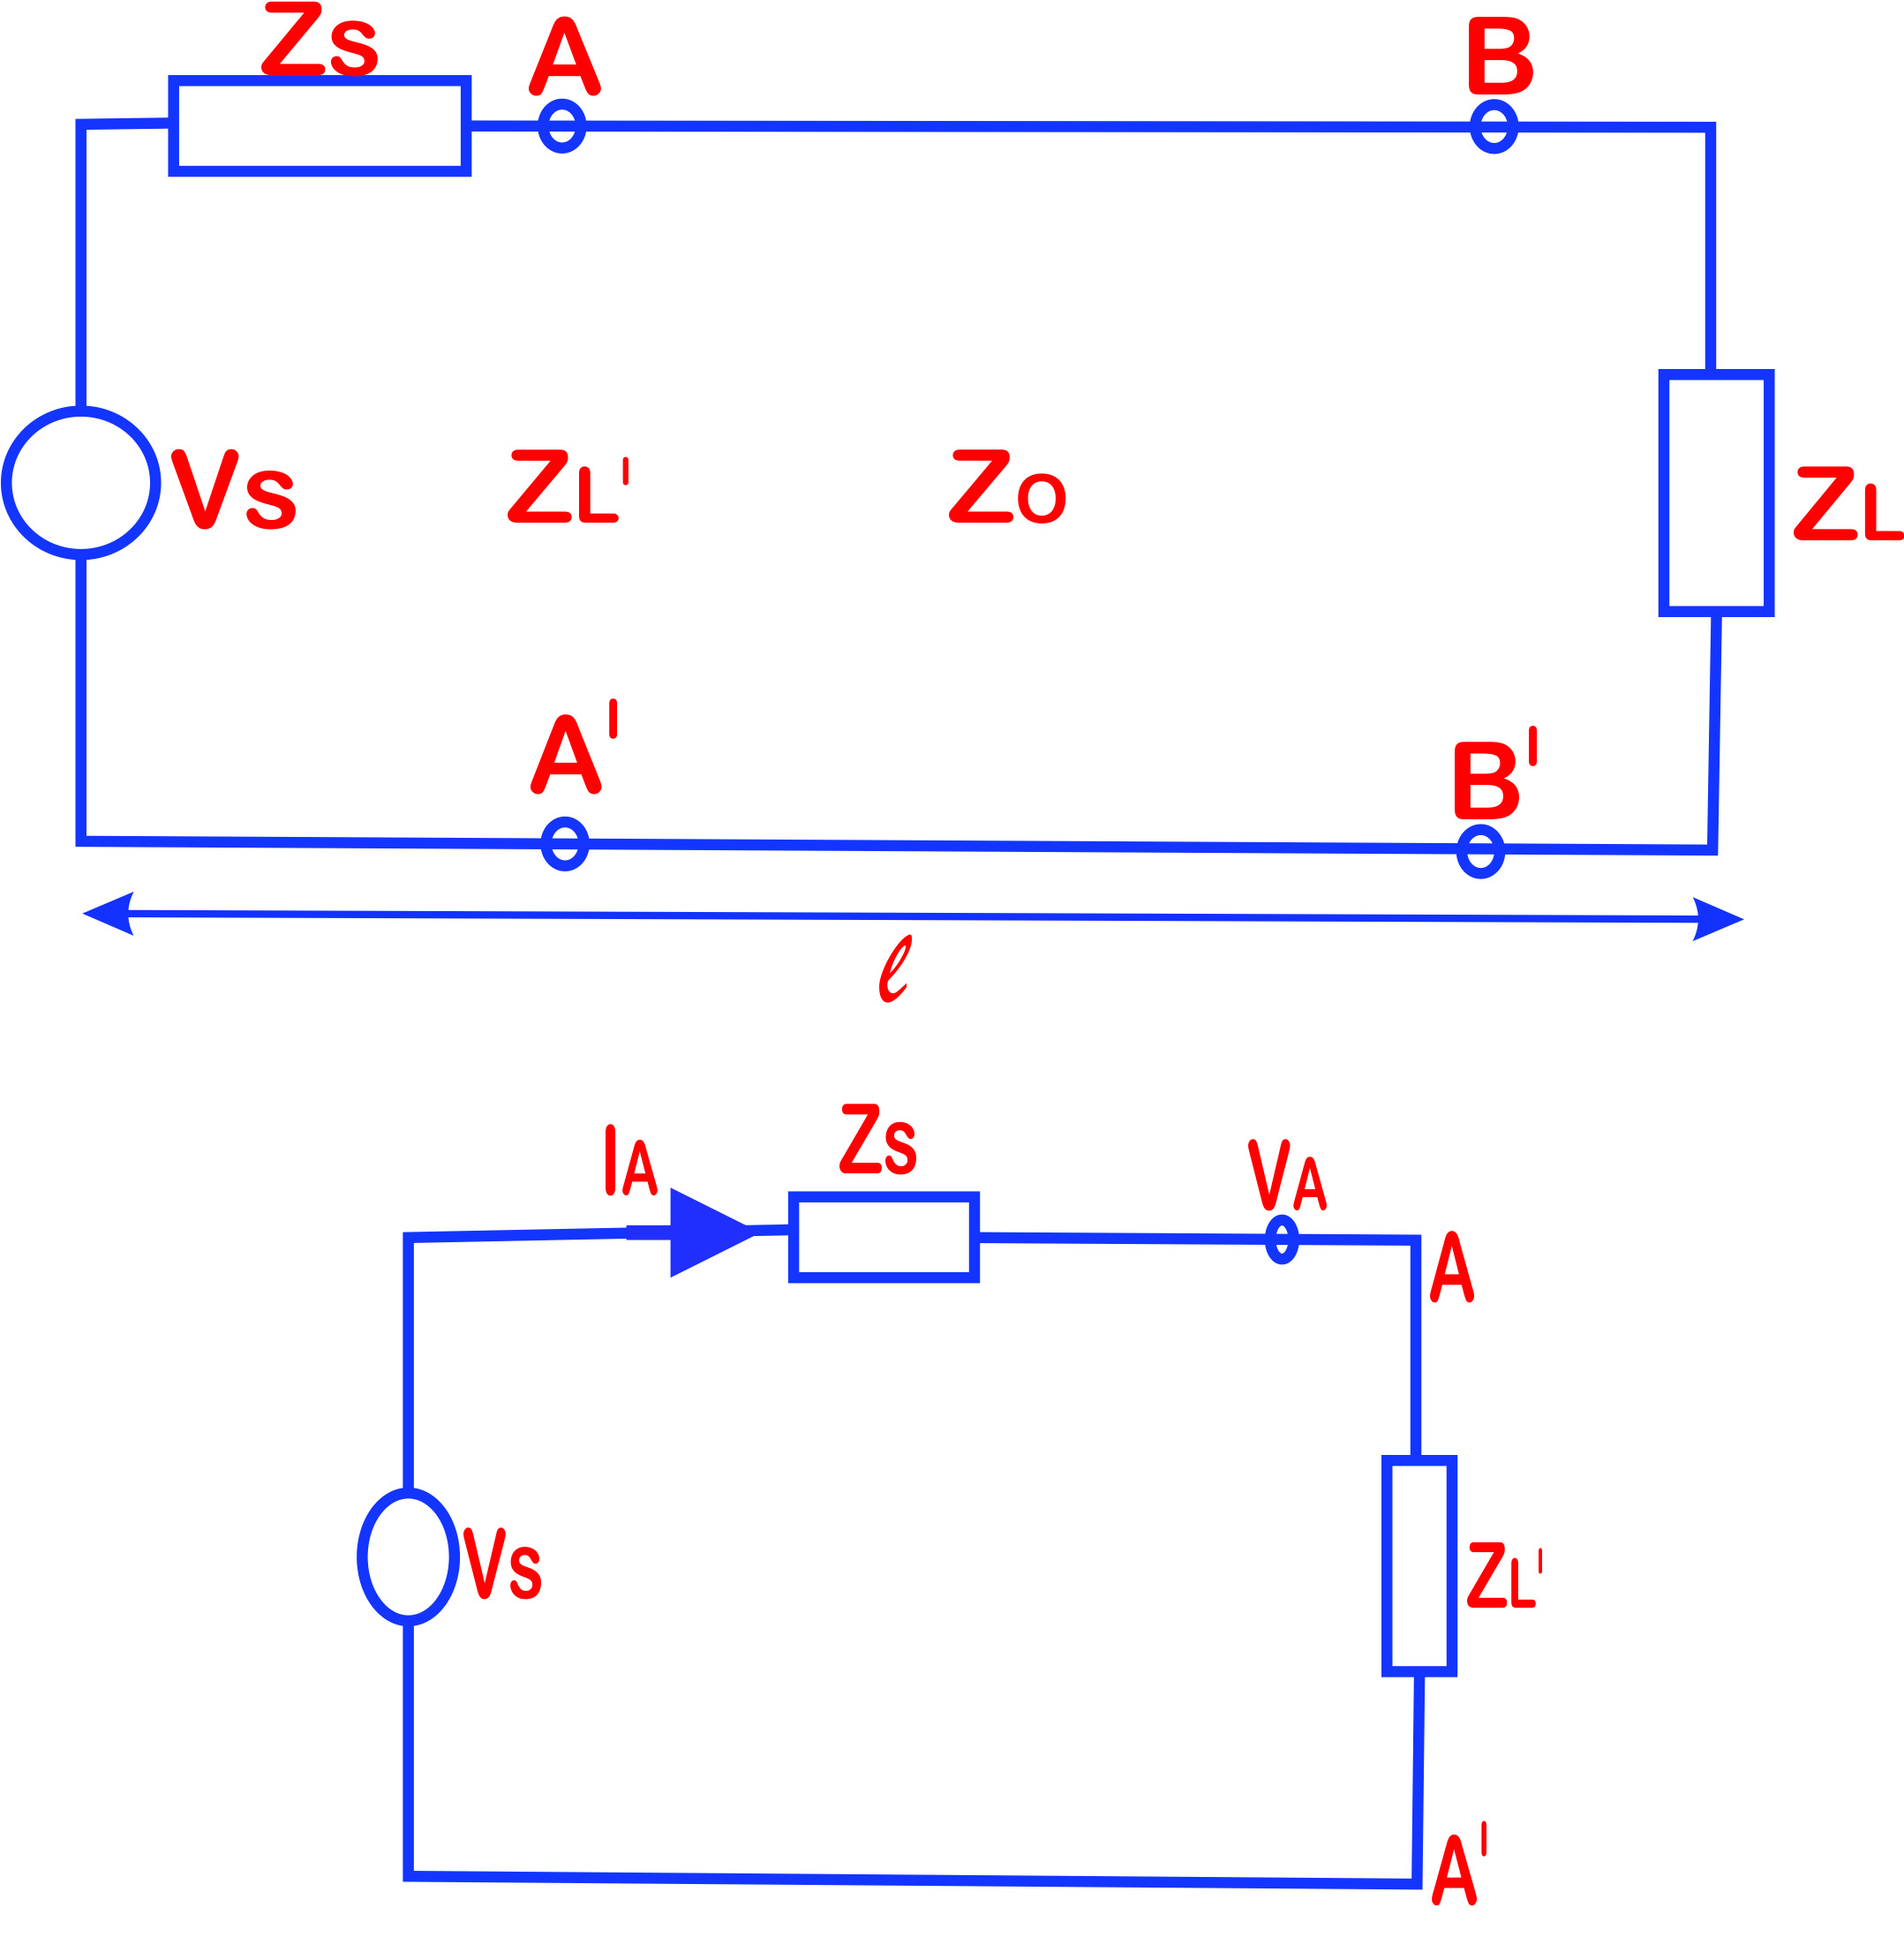
\includegraphics[width=0.7\linewidth]{./graphics/qwerrtt fixed}
\caption{Transformation of load impedance from $Z_L$ to $Z_{L}^'$}
\label{fig:qwerrtt}
\end{figure}

Considering the lumped circuit, the voltage and current equations are\footnote{
The voltage and current relations take the limit as the size of the circuit tends to zero so it is valid for any arbitrary frequency.
}
\begin{align}
V_A &= \frac{Z^'_L}{Z^{'}_L + Z_s} . V_s\label{eqn:transimpvoltage}\\
I_A &= \frac{V_A}{Z^{'}_L}\label{eqn:transimpcurrent}
\end{align} 
We can then determine the voltage and current at the tranformed location using the transmission line equations, such that,
\begin{align*} 
V_A &= V(l) = V^+ e^{j\beta l} \left\lbrace 1 + \Gamma_L e^{-j2\beta l} \right\rbrace\\
I_A &= I(l) = \frac{V^+}{Z_o} e^{j\beta l} \left\lbrace 1 - \Gamma_L e^{-j2\beta l} \right\rbrace
\end{align*}
So we know now the value of $V_A$ and $I_A$ from the lumped element side of view and the transmission line element side of view. We can equate the two to get,
\begin{equation} 
V_A = \frac{Z^{'}_L}{Z^{'}_L + Z_s} . V_s = V^+ e^{j\beta l} \left\lbrace 1 + \Gamma_L e^{-j2\beta l} \right\rbrace\label{eqn:evaluatev+voltage}
\end{equation}
\begin{equation}
I_A = \frac{V_A}{Z^{'}_L} = I(l) = \frac{V^+}{Z_o} e^{j\beta l} \left\lbrace 1 - \Gamma_L e^{-j2\beta l} \right\rbrace
\label{eqn:evaluatev+current}
\end{equation}
So solving equation~\ref{eqn:evaluatev+current} making $V^{+}$ the subject of the formula, we get the expression of $V^+$ as follows. 
\begin{equation} 
V^+ = \frac{Z^{'}_L V_s e^{-j\beta l}}{(Z_S + Z^{'}_L)(1 + \Gamma_L e^{-j2\beta l })}, 
\end{equation}
$\alpha, \beta, l, \Gamma_L$ and $Z_o$ are all known values, so now we have a known value for $V^+$.

From here $V^+$ can be determined and then substituted into the power equation and so power delivered to the load can be calculated or power at any point along the line. This is a complete solution to voltage and current on the transmission line.

\section{Summary}
Table~\ref{tab:transparams} show the transmission line parameters for lossless and low-loss conditions that have been discussed and derived.
\begin{table}[h]
\caption[short]{Transmission line parameters for lossless and low-loss conditions}
\label{tab:transparams}
\begin{tabular}{l c l}
{\bf Lossless}&   	$\leftrightarrow$  & {\bf Low-loss}  \\ 
$\alpha$ = 0 &  & $\alpha = \dfrac{1}{2}R\sqrt{\frac{C}{L}} + \dfrac{1}{2}G\sqrt{\frac{C}{L}}$\\
$\beta = \omega\sqrt{LC}$ & & $\beta = \omega\sqrt{LC}$\\
$\gamma = j\beta$ & & $\gamma = \alpha + j\beta$\\
$Z_o = \sqrt{\frac{L}{C}}$ = real &  & 	$Z_o = \sqrt{\frac{L}{C}}\left(1 - j\frac{R}{2\omega L} - j\frac{G}{2\omega C}\right)$
\end{tabular} 
\end{table} 

Other parameters that are derived are as follows and they apply equally to lossless and low-loss conditions.
\begin{align*}
\Gamma_L = \frac{Z_L - Z_o}{Z_L + Z_o} = \frac{\bar{Z_L} - 1}{\bar{Z_L} + 1} = \frac{V^-}{V^+}
\end{align*}
\begin{align*}
\text{VSWR, }\rho = \frac{1 + |\Gamma_L|}{1 - |\Gamma_L|}
\end{align*}
\begin{align*}
R_\max &= Z_o \left( \frac{1 + |\Gamma_L|}{1 - |\Gamma_L|}\right) = Z_o \rho\\
Z_\max &= \frac{|V_\max|}{|I_\min|}
\end{align*}
\begin{align*}
R_\min &= Z_o \left(\frac{1 - |\Gamma_L|}{1 + |\Gamma_L|}\right) = \frac{Z_o}{\rho}\\
Z_\min &= \frac{|V_\min|}{|I_\max|}
\end{align*}

For Impedance transformation, we have
\begin{align*}
Z(l) &= Z_o\left\lbrace\frac{Z_L\cos\beta l + jZ_o\sin\beta l}{jZ_o\sin\beta l + Z_L\cos\beta l}\right\rbrace\\ 
&= Z_o\left\lbrace\frac{Z_L\cosh\gamma l + Z_o\sinh\gamma l}{Z_o\cosh\gamma l + Z_L\sinh\gamma l}\right\rbrace
\end{align*}

Lastly, the power flow equations
\begin{dmath*}
P_L = \frac{1}{2}\frac{|V^+|}{Z_o}\lbrace 1 - |\Gamma_L|^2\rbrace\quad\text{Real power}
\end{dmath*}
\begin{dmath*}
P(l) = \frac{1}{2}\frac{|V^+|}{Z_o}\lbrace 1 - |\Gamma_L|^2\rbrace - \mathfrak{Im}\lbrace \Gamma_L e^{- j2\beta l}\rbrace\quad\text{Complex power}
\end{dmath*}
\[
V^+ = \frac{Z_L^{'}V_s e^{-j\beta l}}{(Z_s + Z_L^{'})(1 + \Gamma_L e^{-j2\beta l})}
\]
